\section{Модификация проекта <<Изображение проекции полиэдра>>}

\subsection{Постановка задачи}

Модифицируйте эталонный проект таким образом, чтобы определялась и печаталась следующая характеристика полиэдра: сумма площадей граней, все вершины которых-хорошие точки.

После запуска программы, программа вычисляет площадь хороших полигонов
Это задание не требует серьёзной модификации исходного кода, все функции будут вписываться в файл проекта \verb|polyedr.rb|.

\subsection{Решение}

Для выполнения задания необходимо определить хорошую точку в пространстве,если она строго находится вне сферы $x^2+y^2+z^2=1$.И вычислить сумму площадей граней, все вершины которые-хорошие точки.



\subsection{Модификация кода}

Создадим метод модуля.

\begin{small}
\begin{verbatim}
def length
    Math.sqrt(@x*@x + @y*@y + @z*@z)
  end
\end{verbatim}
\end{small}

Создадим метод хорошей вершины.
Вершина называется хорошей если она лежит за пределами сферы.

\begin{small}
\begin{verbatim}
def good?
    @x*@x + @y*@y + @z*@z > 1#
  end
\end{verbatim}
\end{small}

Создадим метод площади грани.

\begin{small}
\begin{verbatim}
def area#метод площади грани
    result = 0.0

    for i in 1 ... (vertexes.size - 1)
      result += triangle_area(vertexes[0], vertexes[i], vertexes[i + 1])
    end

    return 0.5*result
  end 
\end{verbatim}
\end{small}

Создадим метод который вычисляет площадь треугольника.

\begin{small}
\begin{verbatim}
def triangle_area(a, b, c)
    ((b - a).v(c - a)).length
  end
\end{verbatim}
\end{small}

Создадим метод котовый вычисляет площадь грани,если она является хорошей.

\begin{small}
\begin{verbatim}
def good_area
    result = 0.0

    facets.each do |face|
      result += face.area if face.good?
    end

    return result
  end
\end{verbatim}
\end{small}



\newpage
Увидеть работу этой модификации можно на рис.~3.

\begin{figure}[ht!]
\begin{center}
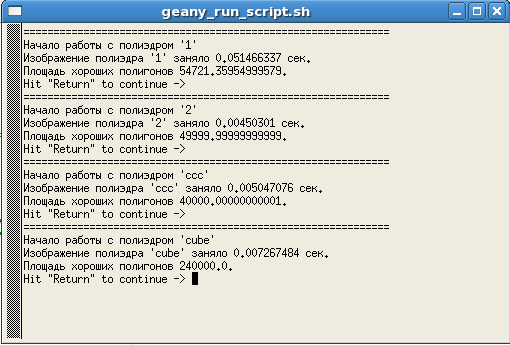
\includegraphics[scale=0.6]{images/5}
\end{center}
\vspace*{-8mm}
\caption{Начало работы с полиэдром 'cube'}\label{fig:term_2}
\end{figure}

Увидеть работу этой модификации можно на рис.~4.

\begin{figure}[ht!]
\begin{center}
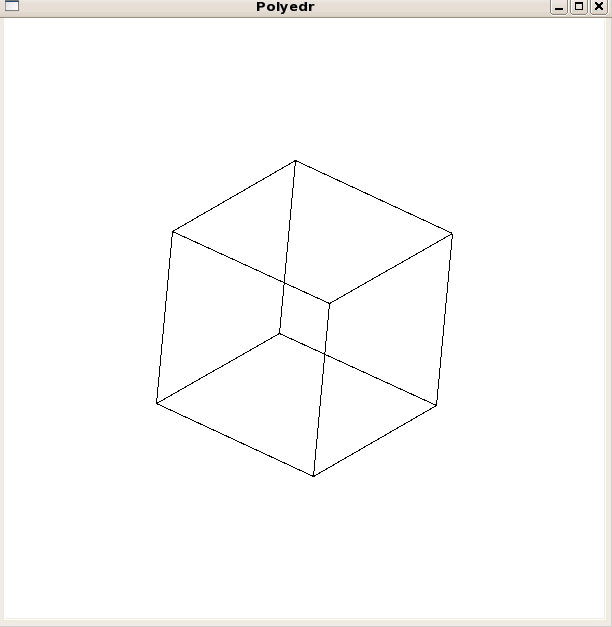
\includegraphics[scale=0.4]{images/4}
\end{center}
\vspace*{-8mm}
\caption{Изображение куба}\label{fig:pic_2}
\end{figure}


